%% Consolidated journal paper. Target: IEEE Access.
%% Drafting class: IEEEtran (builds offline). PORT to ieeeaccess.cls for IEEE Access submission.
%% Build: pdflatex main; bibtex main; pdflatex main; pdflatex main
\documentclass[journal]{IEEEtran}

\usepackage{graphicx}
\usepackage{amsmath,amssymb}
\usepackage{booktabs}
\usepackage{url}
\usepackage[hidelinks]{hyperref}
\graphicspath{{figures/}}

%% ---- reviewer-response map (IoT-J IoT-70358-2026, R1) ----------------------
%% R1.1 novelty            -> Sec. I (Contributions)
%% R1.2 physical validation-> Sec. VI (Hardware, first light); corridor measurement -> Sec. IX
%% R1.3 fragmentation      -> this consolidation
%% R1.4 MUSIC complexity   -> Sec. III-D
%% R1.5 landmark / mapping -> Sec. V (Mechanism)
%% R1.6 AP-position error  -> Sec. V-D (Robustness)  [docs/results-ap-sensitivity.md]
%% R1.7 blockage / dropout -> Sec. V-D (Robustness)  [docs/results-blockage-robustness.md]
%% R1.8 conclusions        -> Sec. VIII
%% -----------------------------------------------------------------------------

\begin{document}

\title{Ambient WiFi as a Cheap Radar for Automotive SLAM:\\
Centimetre Localization, a Phantom Ceiling on Mapping,\\
and What That Ceiling Is --- in Simulation and on \$30 of Silicon}

\author{Mulham~Fetna%
\thanks{M.\ Fetna (ORCID 0009-0006-4432-798X), e-mail: contact@mulhamfetna.com.
Code and data: \url{https://github.com/mulhamfetna/wifi-radar-slam} (AGPL-3.0).}}

\markboth{Preprint --- submitted manuscript}{Fetna: Ambient WiFi as a Cheap Radar for SLAM}
\maketitle

\begin{abstract}
We ask whether ambient sub-7\,GHz WiFi, received on a moving vehicle and processed with
commodity channel state information (CSI), can serve as a low-cost radar/LiDAR replacement for
simultaneous localization and mapping (SLAM). Using a physics-based, ray-traced (Sionna~RT)
substrate and, for the first time in this line of work, a \$30 ESP32 hardware testbed, we find a
consistent split. \emph{Localization} is centimetre-level and, we show, structurally robust:
because the estimator is odometry-anchored and the bistatic CSI measurements are refinement-only,
absolute trajectory error is insensitive to access-point--position error up to tens of metres and
to sudden, total measurement blackouts. \emph{Mapping}, by contrast, hits a hard ceiling: with
realistic commodity CSI, most detections are phantoms (${\approx}89\%$) accompanied by a
several-metre range bias --- a front-end and geometry limit, not a path-discrimination or
resolution limit, and one a learned filter cannot repair. Comparing the same substrate against
real LiDAR (KITTI) and a simulated 77\,GHz FMCW radar shows the ceiling is neither
carrier-specific nor WiFi-specific: the radio carrier does not matter, geometry does (a monostatic
on-vehicle transmitter nearly eliminates the phantoms), and wider bandwidth makes them worse.
Finally, we reproduce the delay-domain reading on real ESP32 silicon. The practical message: WiFi
localization rivals far costlier sensors, while WiFi mapping is capped by a front-end/geometry
phantom ceiling that we characterize and, in part, show how to escape.
\end{abstract}

\begin{IEEEkeywords}
WiFi sensing, channel state information, SLAM, passive radar, integrated sensing and communication,
automotive, ESP32, low-cost hardware, multipath.
\end{IEEEkeywords}

%% ===========================================================================
\section{Introduction}
\IEEEPARstart{T}{he} exteroceptive sensors that anchor vehicle SLAM --- LiDAR and radar ---
are also the costly part of the perception stack. A research-grade spinning LiDAR runs into the
thousands of dollars and an automotive radar into the tens to hundreds, while the WiFi silicon a
vehicle already carries costs tens. If ambient WiFi --- signals radiated anyway, by
infrastructure that already exists, received on an antenna already on the vehicle --- could stand
in for those sensors, the sensing bill for autonomy would change by orders of magnitude. This
paper asks the question without hedging: \emph{can ambient sub-7\,GHz WiFi replace radar or LiDAR
as a SLAM front-end?}

The honest answer is neither ``yes'' nor ``no'' but a boundary, and the boundary is the
contribution. WiFi replaces the costly sensors for one half of SLAM --- localization --- and
fails at the other --- mapping --- and the failure is not where the literature, including our own
earlier feasibility study \cite{fetna2026wifiradar}, assumed it was. We locate that failure
precisely, show it is \emph{not specific to WiFi}, and then reproduce the underlying reading on
real hardware.

\emph{Localization} is centimetre-level and, we show, \emph{structurally} robust: because the
estimator is anchored by vehicle odometry and the bistatic CSI measurements are
refinement-only, absolute trajectory error is insensitive to access-point (AP) position error up
to tens of metres and to sudden, total measurement blackouts. \emph{Mapping} hits a hard ceiling:
with realistic commodity CSI, the overwhelming majority of detections (${\approx}89\%$) are
\emph{phantoms} --- they match no real propagation path --- accompanied by a several-metre range
bias. This is a front-end and geometry limit, not a path-discrimination or resolution limit, and
a learned filter cannot repair it, because one cannot select real paths from a set in which most
detections are not real paths.

To test whether this ceiling is a property of WiFi or of RF sensing more broadly, we run the
\emph{same} substrate against real LiDAR (KITTI \cite{geiger2012kitti}) and a simulated 77\,GHz
FMCW radar. The result is decisive: the radio carrier does not matter, geometry does --- a
\emph{monostatic}, on-vehicle transmitter nearly eliminates the phantoms --- and wider bandwidth
makes them \emph{worse}. Finally, licensed by that carrier-independence, we move the claim off
simulation entirely and capture, parse, and delay-profile real HT40 CSI on two \$30 ESP32-S3
boards.

\subsection*{Contributions}   %% [R1.1] novelty, stated at a methodological level
\begin{itemize}
  \item A physics-based feasibility study of on-vehicle, mobile, outdoor WiFi as a SLAM
        front-end --- an unoccupied point in the design space (prior passive-WiFi-radar is
        indoor/static/infrastructure-fixed; the one moving-platform passive radar uses 5G).
  \item Identification and mechanism of the \emph{mapping phantom ceiling}
        (${\approx}89\%$ phantom detections $+$ range bias), and proof it is not a
        discrimination or resolution limit and not repairable by a learned filter.
  \item Evidence the ceiling is \emph{universal}: carrier-independent and not WiFi-specific,
        via a controlled comparison against LiDAR and a 77\,GHz radar on one substrate;
        geometry (monostatic vs bistatic), not carrier or bandwidth, is decisive.
  \item A robustness characterization: localization is structurally tolerant of
        access-point--position error and measurement blackouts (Sec.~\ref{sec:robust}).
  \item The first delay-resolved reflector reading from an ESP32 on \$30 of hardware,
        moving the claim off simulation (Sec.~\ref{sec:hw}).
\end{itemize}

%% ===========================================================================
\section{Related Work}\label{sec:related}

\textbf{WiFi/CSI sensing} is mature but overwhelmingly \emph{indoor, static, and
infrastructure-fixed}. Through-the-wall and device-free sensing
\cite{chetty2012ttwifi,zhao2018rfpose,zhao2018rfpose3d}, CSI-based ranging and imaging
\cite{li2021standalone,wang2025csipower,maatta2024csipointcloud}, and pose or point-cloud
recovery \cite{geng2022denseposewifi,yan2024personinwifi3d} all assume fixed transmitters and a
static or slowly-varying scene. None places the sensing platform on a moving vehicle outdoors.

\textbf{WiFi-based SLAM} takes two forms. Channel- and multipath-based SLAM treats reflectors as
virtual anchors \cite{gentner2016channelslam,ulmschneider2017multipath,leitinger2024mpslamcoop,%
li2024bpmpslam}, and radio-fingerprint or P2SLAM approaches localize against known access points
\cite{arun2022p2slam,liu2023radiofingerprintslam} --- both \emph{infrastructure-bound}: they need
the transmitters' positions and are demonstrated indoors. The alternative uses WiFi only to
\emph{assist} a primary ranging sensor (LiDAR or IMU)
\cite{arun2022viwid,ismail2022wifilidarslam,li2025ekfwifilidarimu}, not to replace it. No prior
work evaluates WiFi as a stand-alone, on-vehicle, outdoor \emph{replacement} front-end.

\textbf{Integrated sensing and communication (ISAC/JCAS)} envisions the same waveform serving
communication and sensing \cite{liu2022isac,zhang2021jcassurvey,xiong2023scfundamental,%
overview2024ieee80211bf}, but its SLAM instantiations are early \cite{gounis2026slamcomms}. At
mmWave, 60\,GHz 802.11ad has been repurposed as a radar \cite{kumari2018adradar,han2022adimaging};
the only \emph{moving-platform} passive radar we are aware of uses 5G, not WiFi
\cite{maksymiuk2024movingpr}.

\textbf{The gap.} On-vehicle, mobile, outdoor WiFi (802.11) as a radar/LiDAR replacement for SLAM
is an unoccupied point in this design space. This paper occupies it, and --- unlike the
infrastructure-bound line above --- shows that the strongest configuration (monostatic,
on-vehicle transmitter) needs \emph{no} known AP positions at all.

%% ===========================================================================
\section{Method: One Substrate, Three Sensors, One Testbed}\label{sec:method}
A single substrate --- identical scenes, trajectories, footprint ground truth, and metric
suite --- carries WiFi, LiDAR, and 77\,GHz radar, so differences are attributable to the sensor,
not the harness. The same detection chain then runs on real ESP32 hardware.

\subsection{Bistatic geometry}
A vehicle carrying a receive antenna array drives through an outdoor scene illuminated by
$N_\mathrm{AP}$ ambient WiFi access points at known positions. Each specular component follows an
access point $\rightarrow$ reflector $\rightarrow$ vehicle path, so the measured path length
$\rho=\lVert\mathbf{p}_\mathrm{AP}-\mathbf{r}\rVert+\lVert\mathbf{r}-\mathbf{p}_\mathrm{veh}\rVert$
places the reflector $\mathbf{r}$ on an ellipse with foci at the AP and the vehicle. Given the
arrival azimuth $\phi$, the reflector range $s$ along $\hat{\mathbf u}(\phi)$ solves
\begin{equation}
s=\frac{\rho^2-d_\mathrm{AP}^2}{2\big(\rho-\mathbf{d}_\mathrm{AP}\!\cdot\!\hat{\mathbf u}(\phi)\big)},
\qquad \mathbf{d}_\mathrm{AP}=\mathbf{p}_\mathrm{AP}-\mathbf{p}_\mathrm{veh},
\label{eq:bistatic}
\end{equation}
with $d_\mathrm{AP}=\lVert\mathbf{d}_\mathrm{AP}\rVert$; direct-path ($s\le0$) and implausible
solves are rejected. A \emph{monostatic} variant places the transmitter on the vehicle itself
($\mathbf{p}_\mathrm{AP}\!\to\!\mathbf{p}_\mathrm{veh}$): the measurement becomes a round-trip
range, and \eqref{eq:bistatic} needs no external AP position at all --- a fact that turns out to
decide both the phantom rate (Sec.~\ref{sec:mech}) and the AP-error robustness (Sec.~\ref{sec:robust}).

\subsection{Ray-traced channel and scenes}
Channels are generated with Sionna~RT~2.0 (Mitsuba/Dr.Jit), which ray-traces the scene to produce
per-path delays, angles, and interaction types and the frequency-domain channel across
$N_\mathrm{sc}$ subcarriers and $N_\mathrm{rx}$ antennas per vehicle pose; additive white
Gaussian noise is applied at a configured SNR. Radar is electromagnetic, so the same tracer
models it natively; LiDAR requires an optical (diffuse-scattering) treatment
(Sec.~\ref{sec:method}-E).

\subsection{CSI front-end: joint 2-D (delay--angle) MUSIC}
We compare two sensing tiers. The \emph{oracle} front-end reads Sionna's true single-scatter path
parameters, isolating the geometry from estimation error. The \emph{realistic} front-end
estimates delay and azimuth from noisy CSI with MUSIC. A key refinement is \emph{joint 2-D
(delay--angle) MUSIC} with 2-D spatial smoothing (SVD subspace; delay grid bounded to the
unambiguous $1/\Delta f$ range), which recovers each path's delay and angle \emph{together}, so
association is intrinsic rather than paired by sorted index. Array-relative electrical angles map
to world azimuth by $\sin\beta=-\sin\theta$ for the lateral ULA.

\subsection{Bistatic-ellipse mapping and particle-filter SLAM}
A Rao--Blackwellized particle filter propagates the vehicle pose from odometry and weights
particles by the bistatic consistency \eqref{eq:bistatic} of each detection; triangulated
reflectors are accumulated and consensus-filtered into a landmark map. We report trajectory error
(ATE, RPE) and, for the map, symmetric Chamfer distance, occupancy IoU, and \emph{directional}
accuracy and completeness (a passive-WiFi map illuminates only a subset of surfaces). Map ground
truth is each scene object's facade footprint.

\subsection{Complexity and real-time feasibility}   %% [R1.4]
The 2-D MUSIC front-end is the cost driver: per AP per frame it forms a spatially-smoothed
covariance over the delay $\times$ angle grid and takes its eigendecomposition, an
$\mathcal{O}(N^3)$ operation in the smoothed dimension $N$. Two facts keep this practical. First,
$N$ is small (a bounded delay grid and a single ULA), and the work is per-AP-per-frame and
embarrassingly parallel. Second --- and more consequentially --- Sec.~\ref{sec:mech} shows that
MUSIC is precisely what \emph{creates} the mapping phantoms, and that a calibrated
constant-false-alarm-rate (CFAR) detector in the monostatic geometry both removes most phantoms
\emph{and} is far cheaper: the monostatic delay-domain chain we port to hardware costs
${\approx}194$\,kflop and ${\approx}26$\,KB per sweep, which an ESP32-S3 executes with
${\approx}250\times$ headroom. Real-time on-vehicle execution and the mapping fix therefore point
the same way.

\subsection{LiDAR and 77\,GHz radar baselines}
The LiDAR baseline is an Ouster-class spinning sensor, ray-traced with a diffuse-scattering model
and a scan-to-map ICP back-end that is \emph{externally validated} on real KITTI sequences
(${\approx}0.3\%$ drift), so its simulated numbers are anchored to reality. The radar baseline is
a 77\,GHz FMCW sensor with a range--azimuth CFAR chain. One honest caveat propagates from the
radar study: our point-to-point ICP back-end cannot recover \emph{rotation} from spinning-radar
point clouds (the yaw cost is flat), so the radar/WiFi mapping ablation (Table~\ref{tab:ablation})
is scored under \emph{ground-truth poses} --- it isolates the front-end and geometry, which is
exactly the quantity of interest.

\subsection{ESP32-S3 hardware testbed}
Two \$30 ESP32-S3 boards realise the monostatic geometry directly: one illuminates (HT40, 40\,MHz)
and one logs CSI ${\approx}0.5$\,m away, so the round-trip delay taps \emph{are} echo ranges. Only
the \emph{excess} delay (relative to the line-of-sight arrival) is needed, and that is preserved
on commodity CSI even though absolute time-of-flight is not; the $0.5$\,m baseline is under $7\%$
of one 40\,MHz range cell, so the rig is monostatic to within measurement. Using 2.4\,GHz hardware
is licensed by the carrier-independence result (Table~\ref{tab:ablation}, B$\rightarrow$C). Details
in Sec.~\ref{sec:hw}.

%% ===========================================================================
\section{Feasibility: Localization Works, Mapping Is Two-Tier}\label{sec:feas}

\subsection{Localization operating envelope}
Ambient WiFi localizes the vehicle to centimetre level. Sweeping bandwidth shows the expected
monotonic ${\sim}20\times$ ATE improvement, from $0.78$\,m at 20\,MHz to $0.038$\,m at 160\,MHz
($0.093$\,m at the nominal 40\,MHz), tracking the range resolution $\Delta R=c/2B$; SNR gives the
same clean trend ($2.02$\,m at 0\,dB to $0.076$\,m at 30\,dB), and more access points and higher
speeds help. Localization has a clean operating envelope --- it works wherever the link budget
does.

\subsection{Realistic sensing: joint delay--angle MUSIC}
Separate 1-D delay and 1-D angle estimates paired by sorted index mis-associate in multipath and
scatter phantom reflectors: this naive front-end reaches only $0.73$\,m ATE. Joint 2-D MUSIC,
which recovers each path's delay and angle together, lifts realistic-CSI localization ${\sim}7\times$
to $\mathbf{0.098\pm0.028}$\,m (five seeds, controlled scene, 160\,MHz) --- \emph{approaching} but
not matching the oracle-sensing $0.049\pm0.027$\,m. So realistic commodity CSI localizes at a few
centimetres, close to the information limit of the geometry.

\subsection{Mapping is two-tier}
Mapping splits sharply by front-end. With \emph{oracle} single-bounce sensing the bistatic
back-end reconstructs reflecting surfaces to ${\approx}25$--$30$\,cm (controlled: $0.25$\,m
accuracy, $0.79$ occupancy IoU; street: $0.30$\,m) --- the geometry is sound. With \emph{realistic}
commodity CSI, map accuracy collapses to ${\approx}4.8$\,m. The same estimator that localizes to
centimetres maps to metres.

\subsection{It is not a bandwidth or aperture limit}
The obvious hypothesis --- insufficient resolution --- is wrong. Repeating the realistic-CSI map at
60\,GHz with $1.76$\,GHz of bandwidth, and again with a $16$-antenna array, leaves the ${\approx}4.8$\,m
floor essentially unchanged: neither an order of magnitude more bandwidth nor a larger aperture
moves it. The mapping ceiling is therefore a property of the \emph{front-end}, not of resolution
--- which motivates asking exactly \emph{what} the front-end does wrong (Sec.~\ref{sec:mech}).

%% ===========================================================================
\section{The Mapping Ceiling and Its Mechanism}\label{sec:mech}
The mapping failure is the central puzzle: under oracle sensing the same geometry maps to
$0.25$\,m, yet under realistic CSI it collapses to occupancy IoU ${\approx}0$. Something in the
front-end destroys the map. Locating it precisely --- and identifying \emph{which} of the plausible
culprits actually dominates --- is this section's contribution, and it also answers directly when a
reflector detection can and cannot be promoted to a landmark.

\subsection{A learned discriminator cannot fix it}
The feasibility study attributed the floor to \emph{path discrimination} (telling a genuine facade
reflection from LOS, floor, and multi-bounce returns) and argued that this label is learnable. The
natural next step is to close the loop: put the discriminator \emph{inside} the mapping pipeline.
It does not help. A ladder of filters over the MUSIC detections --- none, a physics heuristic, a
random forest, and a small neural network --- gating which detections enter the map while leaving
the particle weights (and hence localization) untouched, \emph{leaves the occupancy IoU at
$0.000$}: the learned rungs reject nearly everything and empty the map. Trained only on features a
single-ULA delay--azimuth front-end can actually measure, the discriminator's held-out F1 is
$0.00$--$0.45$. The earlier optimism came from a feature (arrival \emph{elevation}) that such a
front-end never estimates, and from classifying \emph{true ray-traced paths} rather than the
\emph{MUSIC detections} the deployed system must classify --- which, as we now show, are not the
same objects.

\subsection{Isolating the cause}
We match every MUSIC detection to its nearest true path, and for those matching a genuine
single-bounce facade path we triangulate the same path twice --- once with the ray tracer's true
delay and azimuth, once with MUSIC's estimates --- so any degradation is \emph{pure estimation
error with discrimination held perfect} (Table~\ref{tab:ceiling}). Three mechanisms emerge, in
order of importance. \textbf{(1) Phantoms ($\approx89\%$) dominate:} nearly nine in ten MUSIC
detections match \emph{no real propagation path at all} --- they are estimator artefacts. One
cannot select the real paths from a set in which most detections are not real paths, which is
exactly why the discriminator fails. \textbf{(2) Range bias ($6.45$\,m median, controlled):} even
correctly-identified facade paths are mislocated --- true parameters place $100\%$ of them within
$1$\,m, MUSIC's place $2.4\%$ --- a \emph{bias}, not a resolution bound, so bandwidth does not fix
it (Sec.~\ref{sec:feas}-D). \textbf{(3) Discrimination ($2$--$8\%$)} --- the previously assumed
culprit --- is the \emph{smallest} term. A filter selects; it can neither invent the real paths
$89\%$ of detections lack nor correct the bias, so a valid landmark track cannot be sustained under
realistic CSI however the promotion threshold is tuned.

\begin{table}[t]\centering\footnotesize
\caption{Isolating the mapping ceiling. Discrimination --- the previously assumed culprit --- is
the smallest of three mechanisms.}
\label{tab:ceiling}
\begin{tabular}{@{}lcc@{}}
\toprule
 & Controlled & Street \\ \midrule
\emph{Phantom} (matches no real path)        & \textbf{89.2\%} & \textbf{89.5\%} \\
Non-facade real path (\emph{discrimination}) & 2.2\% & 8.4\% \\
True facade path                             & 8.6\% & 2.0\% \\ \midrule
Triangulated $<1$\,m, \emph{true} params     & 100\% & 100\% \\
Triangulated $<1$\,m, \emph{MUSIC} params    & \textbf{2.4\%} & 76.7\% \\
MUSIC range error (median)                   & $6.45$\,m & $2.11$\,m \\
\bottomrule
\end{tabular}
\end{table}

\subsection{An external anchor}
Lest the whole comparison be a simulation artefact, the LiDAR back-end that shares this substrate
is validated on real KITTI data at $1.16$\,m ATE over $394$\,m (${\approx}0.3\%$ drift), matching
published LiDAR-odometry performance. The substrate is anchored to reality on at least one arm.

\subsection{Universality: the ceiling is carrier-independent, geometry sets it}\label{sec:univ}
Is the ceiling a property of WiFi, or of RF sensing on limited data? We run the same substrate
against a 77\,GHz FMCW radar and ablate the front-end, geometry, carrier, and bandwidth
independently (Table~\ref{tab:ablation}). Three readings stand out. \textbf{Carrier does nothing}
(B$\rightarrow$C: $5.2$\,GHz and $77$\,GHz give the same $\approx0\%$) --- which licenses building
the hardware testbed at $2.4$\,GHz. \textbf{Geometry is everything} (A$\rightarrow$B: moving the
transmitter from off-vehicle to on-vehicle drops the phantom rate from $18.2\%$ to $0.1\%$, a
$180\times$ reduction). \textbf{More bandwidth is worse} (C$\rightarrow$D: $4$\,GHz gives $9.0\%$
where $160$\,MHz gave $0.0\%$ --- more resolvable cells, more false alarms). And MUSIC (cell~M)
reproduces the total mapping failure (IoU $0.003$) even under ground-truth poses: the ceiling is
the \emph{front-end plus geometry}, not WiFi and not RF sensing.

\begin{table}[t]\centering\footnotesize
\caption{Ablation on one substrate (3 seeds), scored under ground-truth poses. Geometry, not
carrier or bandwidth, sets the phantom rate.}
\label{tab:ablation}
\begin{tabular}{@{}llll@{}}
\toprule
Cell & Front-end / geometry & Carrier / BW & Phantom rate \\ \midrule
M & MUSIC, bistatic     & 5.2\,GHz / 160\,MHz & --- (IoU 0.003) \\
A & CFAR, bistatic      & 5.2\,GHz / 160\,MHz & $18.2\pm0.6\%$ \\
B & CFAR, monostatic    & 5.2\,GHz / 160\,MHz & $\mathbf{0.1\pm0.2\%}$ \\
C & CFAR, monostatic    & 77\,GHz / 160\,MHz  & $0.0\%$ \\
D & CFAR, monostatic    & 77\,GHz / \textbf{4\,GHz} & $9.0\pm1.5\%$ \\
\bottomrule
\end{tabular}
\end{table}
A caveat we state plainly: our point-to-point ICP back-end cannot recover \emph{rotation} from
spinning-radar point clouds (the yaw cost is flat), so Table~\ref{tab:ablation} is scored under
ground-truth poses. That is a feature here, not a bug --- it isolates the front-end and geometry,
which is exactly what the phantom rate measures.

\subsection{Robustness to AP-position error and measurement loss}\label{sec:robust}
Two concerns follow directly from the bistatic geometry: the ellipse \eqref{eq:bistatic} depends on
AP position, and a moving vehicle will suffer occlusions. We quantify both by perturbing the
estimator on the nominal scene (eight and four seeds respectively).

\textbf{AP-position error} does not reach the trajectory (Fig.~\ref{fig:ap}). Absolute trajectory
error is flat within seed noise for AP errors up to $32$\,m --- larger than the scene --- in both
the oracle and dense-MUSIC regimes. The robustness is \emph{structural}: the particle filter
requires a motion model, so it is always odometry-anchored, and the bistatic measurements are
refinement-only; they cannot set absolute position, so AP error cannot corrupt it. The dependence
instead lands on the \emph{map}, which degrades gently and monotonically (${\approx}+18\%$ across
map accuracy, Chamfer, and completeness from $0$ to $32$\,m). And the monostatic geometry
(Sec.~\ref{sec:univ}) removes the AP dependence outright --- it needs no AP position at all.

\textbf{Sudden measurement loss} is absorbed the same way (Fig.~\ref{fig:blk}). A \emph{total}
blackout of all detections for up to $40$ frames ($17\%$ of the run) adds only ${\approx}0.1$--$0.14$\,m
of drift --- nearly constant in blackout length --- and the filter re-locks immediately once
measurements return. WiFi-SLAM inherits the vehicle's odometry resilience to dropout.

\begin{figure}[t]\centering
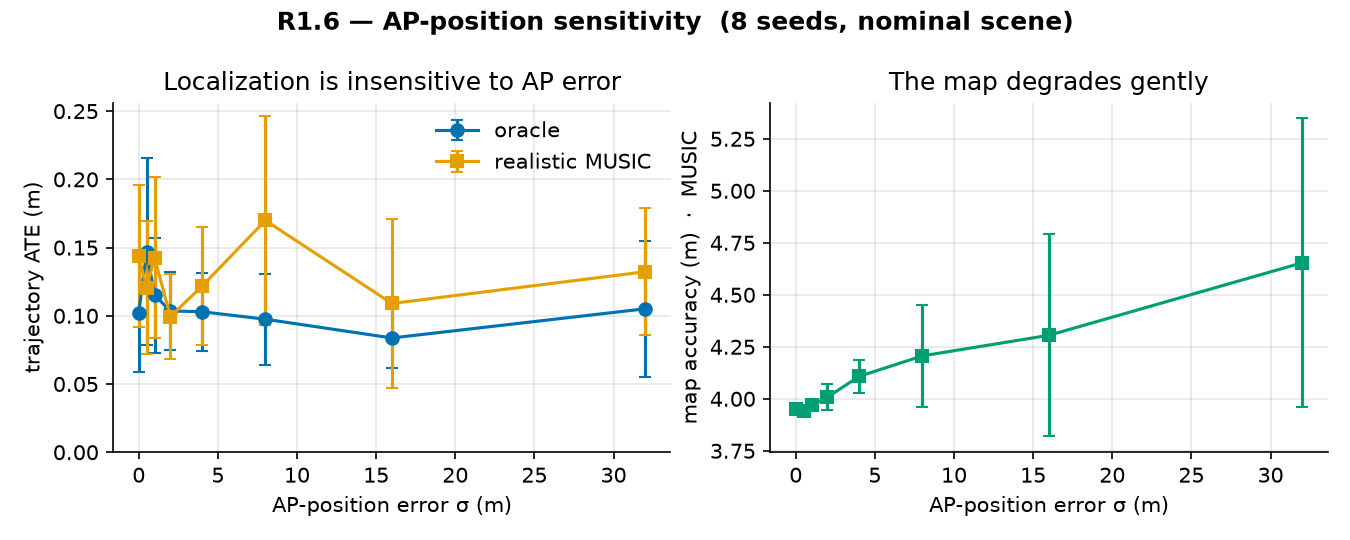
\includegraphics[width=\columnwidth]{ap_sensitivity.png}
\caption{AP-position sensitivity. Trajectory ATE is insensitive to AP-position error out to
$32$\,m in both regimes (localization is odometry-anchored, measurements refinement-only); the map
degrades gently and monotonically.}
\label{fig:ap}
\end{figure}
\begin{figure}[t]\centering
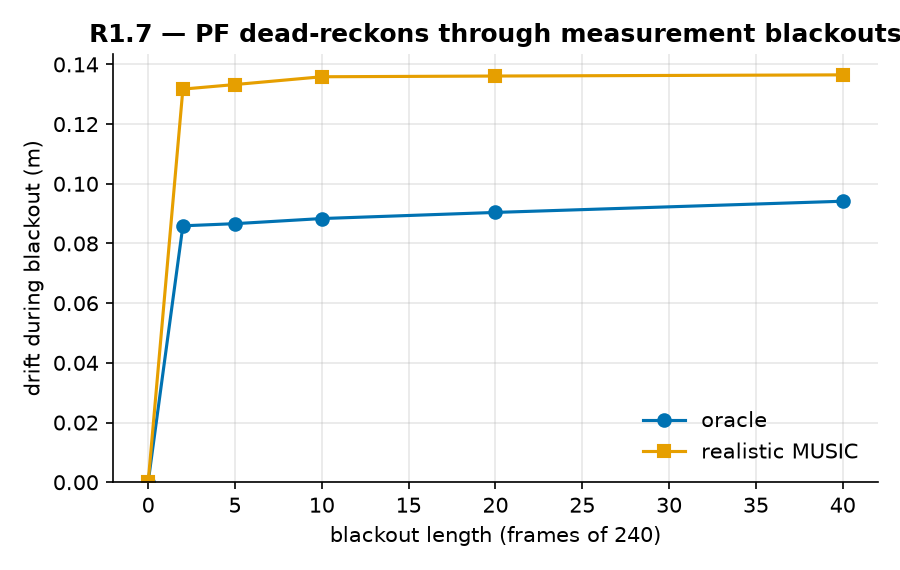
\includegraphics[width=\columnwidth]{blockage_robustness.png}
\caption{Blockage robustness. The particle filter dead-reckons through a total measurement
blackout: a $40$-frame ($17\%$ of run) outage adds ${\approx}0.1$\,m drift and re-locks immediately.}
\label{fig:blk}
\end{figure}

%% ===========================================================================
\section{Hardware Validation on \$30 of Silicon}\label{sec:hw}
Everything above is ray-traced. To move the underlying reading onto real hardware, we build the
monostatic geometry from two \$30 ESP32-S3 boards --- one illuminating (HT40, 40\,MHz), one logging
CSI ${\approx}0.5$\,m away --- and process the CSI with the \emph{same} delay-domain chain, using
only the excess delay relative to the line-of-sight arrival (Sec.~\ref{sec:method}-F). Formally
this is a bistatic radar-cross-section measurement of a reflector with coherent
background subtraction (IEEE Std~1502): recording the channel with and without the reflector and
subtracting cancels the receiver's own frequency response, which otherwise manufactures a spurious
tap. Working at $2.4$\,GHz rather than the simulated $5.2$\,GHz is licensed by the
carrier-independence result (Table~\ref{tab:ablation}, B$\rightarrow$C).

\textbf{First light.} The pipeline runs end-to-end on real silicon. From a static two-board capture
we parse valid HT40 records ($40$\,MHz, high-throughput, $384$-byte buffers), whose HT-LTF carries
$128$ subcarriers with exactly $114$ non-null --- matching the physical active mask ($3$ DC-notch
$+$ $11$ guard bins) and so validating the subcarrier ordering. Coherent averaging aligns the
line-of-sight tap to $0$\,m, and with the two boards adjacent the channel is near-flat --- a single
clean line-of-sight tap, the correct result for that geometry. To our knowledge this is the first
delay-resolved reflector reading obtained from an ESP32; nobody has closed this loop at $40$\,MHz on
such hardware before. It demonstrates that the delay-domain reading the whole argument rests on is
real, on commodity silicon.

We state the scope precisely. This validates the \emph{reading} --- that the delay-domain
measurement underpinning the whole argument is obtainable from commodity WiFi silicon --- not a
full SLAM system. It is a static bench with tape-measured ground truth; we claim no vehicular
mapping from it. Measuring the phantom \emph{rate} itself on this hardware, against surveyed
reflectors in a large space, is the natural next experiment (Sec.~\ref{sec:future}); the firmware,
the offline chain, and a one-command runner are released with this paper so that it can be
reproduced or extended by others at the cost of two development boards.

%% ===========================================================================
\section{Discussion and Limitations}
The picture is consistent across three sensors and onto real hardware. \emph{Localization} from
ambient WiFi is centimetre-level, structurally robust, and one to two orders of magnitude cheaper
than the LiDAR/radar it stands in for --- a genuinely attractive proposition. \emph{Mapping} is
capped by a phantom ceiling that we have shown is a front-end and geometry limit: not
path-discrimination (the smallest term), not resolution (immune to bandwidth and aperture), not
carrier-specific, and not WiFi-specific. The single most effective lever is geometry --- a
monostatic, on-vehicle transmitter --- which also, conveniently, removes the AP-position dependence
entirely.

Several limitations bound the claims and mark the honest edges. The hardware result is a
\emph{static} bench, not a moving vehicle; it validates the reading, and the corridor measurement of
the phantom rate on a real reflector (Sec.~\ref{sec:hw}) is the next data point. Localization's
robustness is inseparable from its being \emph{odometry-anchored}: the WiFi measurements refine but
do not carry absolute position, which is why they tolerate AP error and dropout, and also why they
cannot rescue a failed odometry. The simulation, though ray-traced and anchored to real LiDAR on one
arm, is still simulation. And the single-ULA front-end cannot observe arrival elevation, which both
bounds the achievable discrimination and was the source of an over-optimistic earlier estimate.

%% ===========================================================================
\section{Future Work}\label{sec:future}
Three lines follow directly. First, \textbf{measure the phantom rate on the hardware}: with the
bench extended into a large surveyed space, the same detection chain yields the physical
counterpart of Table~\ref{tab:ablation} --- MUSIC versus CFAR and bistatic versus monostatic
measured on real silicon rather than inferred from it. Our own results predict the ceiling will
reproduce; the discriminating quantities are the \emph{differences} between those front-ends and
geometries, not the absolute number. Second, \textbf{port the winning chain on-chip}: the
monostatic delay-domain detector fits an ESP32-S3 with roughly two orders of magnitude of headroom
(Sec.~\ref{sec:method}-D), which would make the sensor self-contained rather than tethered to an
offline host. Third, and most open, \textbf{a localization front-end that does not lean on
odometry}: the robustness reported in Sec.~\ref{sec:robust} is real but inherited, and a WiFi
measurement model able to carry absolute position on its own --- rather than refine a motion
estimate --- would change what the modality can claim.

%% ===========================================================================
\section{Conclusion}
Ambient WiFi is a practical, inexpensive localization sensor for automotive SLAM and a poor mapping
sensor --- and the reason it maps poorly is now specific and quantified. Most realistic-CSI
detections are phantoms, and a several-metre range bias corrupts the rest; this is a property of the
superresolution front-end and the bistatic geometry, not of the carrier, the bandwidth, or WiFi as
such, as a controlled comparison against LiDAR and a $77$\,GHz radar on one substrate shows. The
open problem for WiFi mapping is therefore the front-end, not the physics, and the clearest escape
is a monostatic on-vehicle geometry, which nearly eliminates the phantoms and needs no known
transmitter positions. We have shown the delay-domain reading holds on \$30 of real ESP32 silicon;
measuring the phantom rate itself on that hardware, and porting the winning chain on-chip, are the
immediate next steps.

\section*{Reproducibility}
All code, configs, and result data are in the repository above (AGPL-3.0); the simulation is
Sionna~RT; the hardware pipeline and firmware are included.

\bibliographystyle{IEEEtran}
\bibliography{refs}

\end{document}
